\documentclass[xcolor=x11names,compress]{beamer}
\usepackage[english]{babel}

%% General document %%%%%%%%%%%%%%%%%%%%%%%%%%%%%%%%%%
\usepackage{graphicx}
\usepackage{tikz}
\usepackage{wrapfig}

\usetikzlibrary{decorations.fractals}
%%%%%%%%%%%%%%%%%%%%%%%%%%%%%%%%%%%%%%%%%%%%%%%%%%%%%%


%% Beamer Layout %%%%%%%%%%%%%%%%%%%%%%%%%%%%%%%%%%
\useoutertheme[subsection=false,shadow]{miniframes}
\useinnertheme{default}
\usefonttheme{serif}
\usepackage{palatino}

\setbeamerfont{title like}{shape=\scshape}
\setbeamerfont{frametitle}{shape=\scshape}

\setbeamercolor*{lower separation line head}{bg=DeepSkyBlue4} 
\setbeamercolor*{normal text}{fg=black,bg=white} 
\setbeamercolor*{alerted text}{fg=red} 
\setbeamercolor*{example text}{fg=black} 
\setbeamercolor*{structure}{fg=black} 
 
\setbeamercolor*{palette tertiary}{fg=black,bg=black!10} 
\setbeamercolor*{palette quaternary}{fg=black,bg=black!10} 

\renewcommand{\(}{\begin{columns}}
\renewcommand{\)}{\end{columns}}
\newcommand{\<}[1]{\begin{column}{#1}}
\renewcommand{\>}{\end{column}}
%%%%%%%%%%%%%%%%%%%%%%%%%%%%%%%%%%%%%%%%%%%%%%%%%%
\newcommand{\hlb}[1]{\textbf{\textcolor{blue}{#1}}}
\newcommand{\hl}[1]{\textcolor{blue}{#1}}
\newcommand{\lien}[2]{\mathcal{L}_{#1}^{#2}}
\newcommand{\lie}[1]{\mathcal{L}_{#1}}

%\usepackage[english]{babel}
\usepackage[utf8]{inputenc}
%\usetheme{Goettingen}

\begin{document}
\title{Bifurcations in continuous time dynamical systems}
\author{Debsankha Manik}

\begin{frame}

%opening

\titlepage

\end{frame}


\section{Grazing}

\begin{frame}{Grazing}

\begin{figure}
\caption{Poincare section for grazing orbit}
\begin{center}
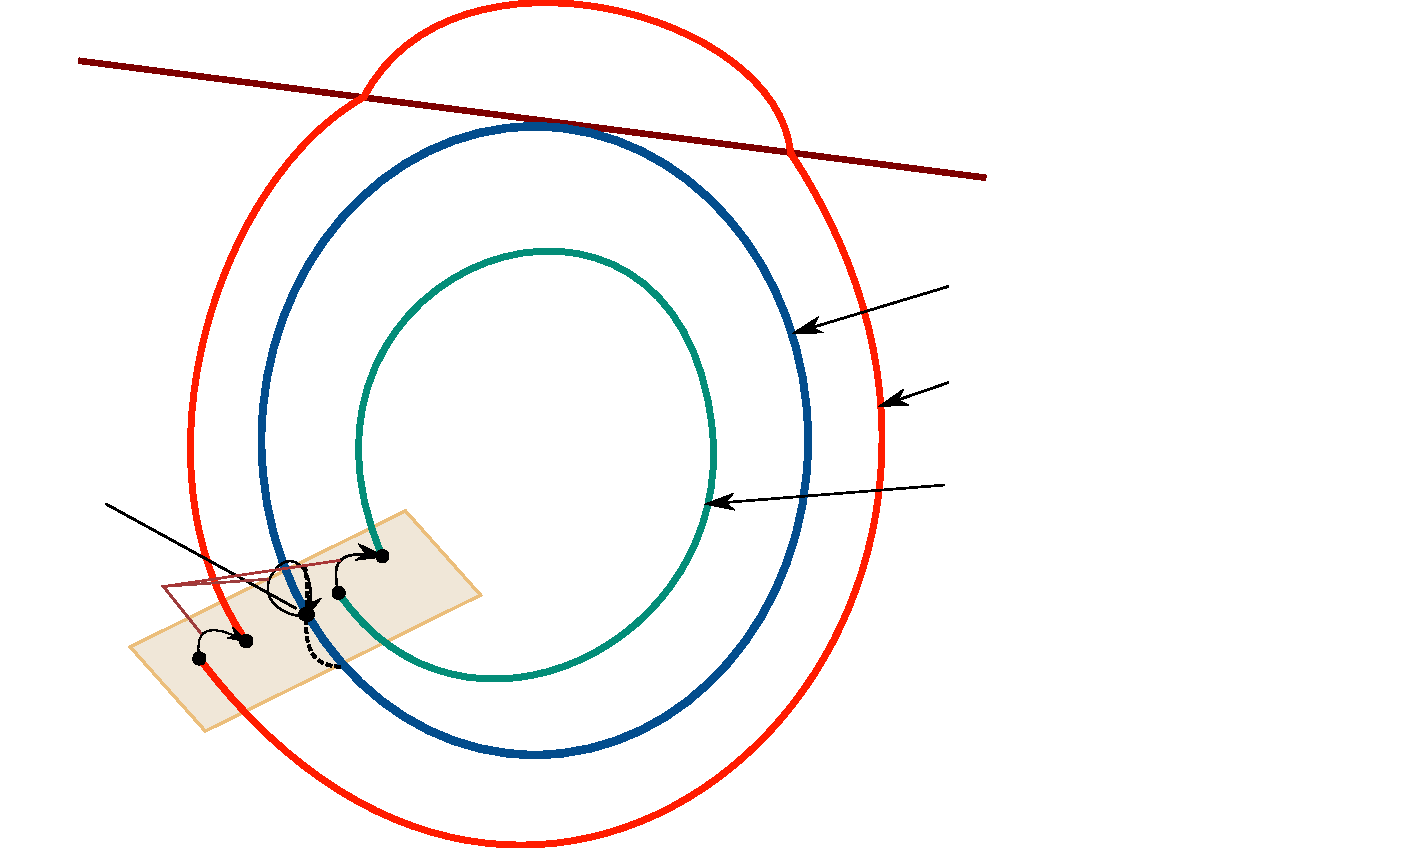
\includegraphics[height=0.7\textheight]{graz}
\end{center}
\end{figure}
\end{frame}

\begin{frame}{Prpperties of grazing orbit}
Let the grazing take place at $x=0$.  
\begin{itemize}
\item $H(0)=0$
\item $\frac{dH}{dx}\neq 0$
\item $\frac{d}{dt}\left.  H(\varphi_i(o,t))\right|_{t=0}=0$
\item $a_i:=\frac{d^2}{dt^2}\left.  H(\varphi_i(o,t))\right|_{t=0}>0$
\end{itemize}
\end{frame}

\section{ZDM-Intro}
\begin{frame}{}

\begin{figure}
\caption{What is ZDM?}
\begin{center}
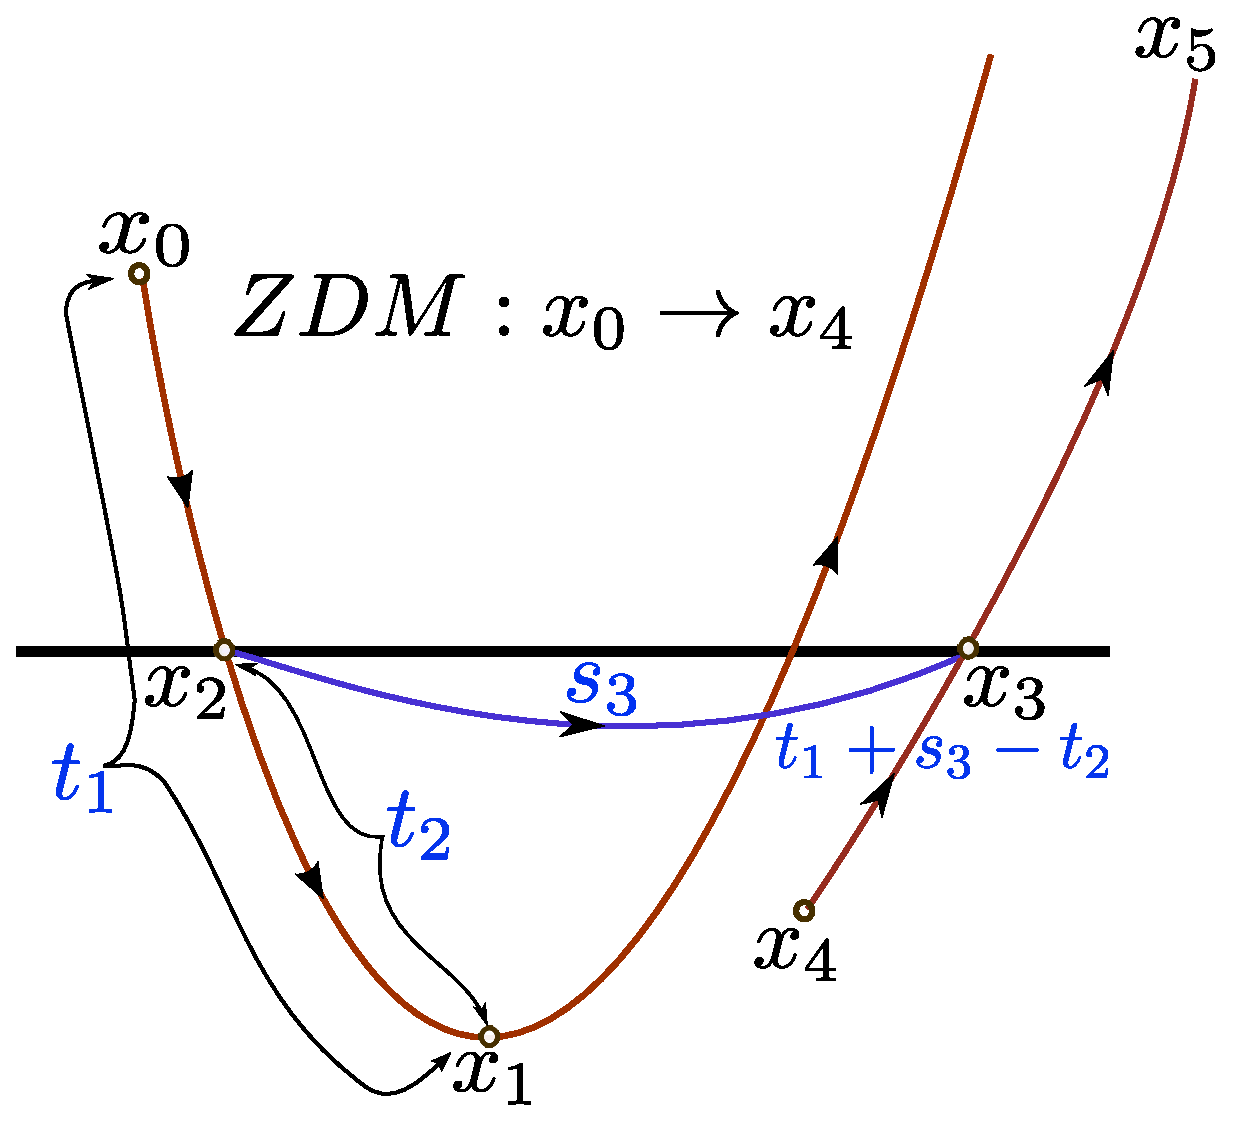
\includegraphics[width=0.7\columnwidth]{ZDM}
\end{center}
\end{figure}

\end{frame}


\begin{frame}{Why the ZDM?}

\hlb{ Why ZDM?}\\
Consider a Poincare section $t\bmod T=0$. Then the Poincare map would be 
simplified to:\\
\[
f(x_n)=\varphi_2(ZDM(\varphi_1(x_n,\tau_0)),T-\tau_0)
\] 
\begin{figure}
\begin{center}
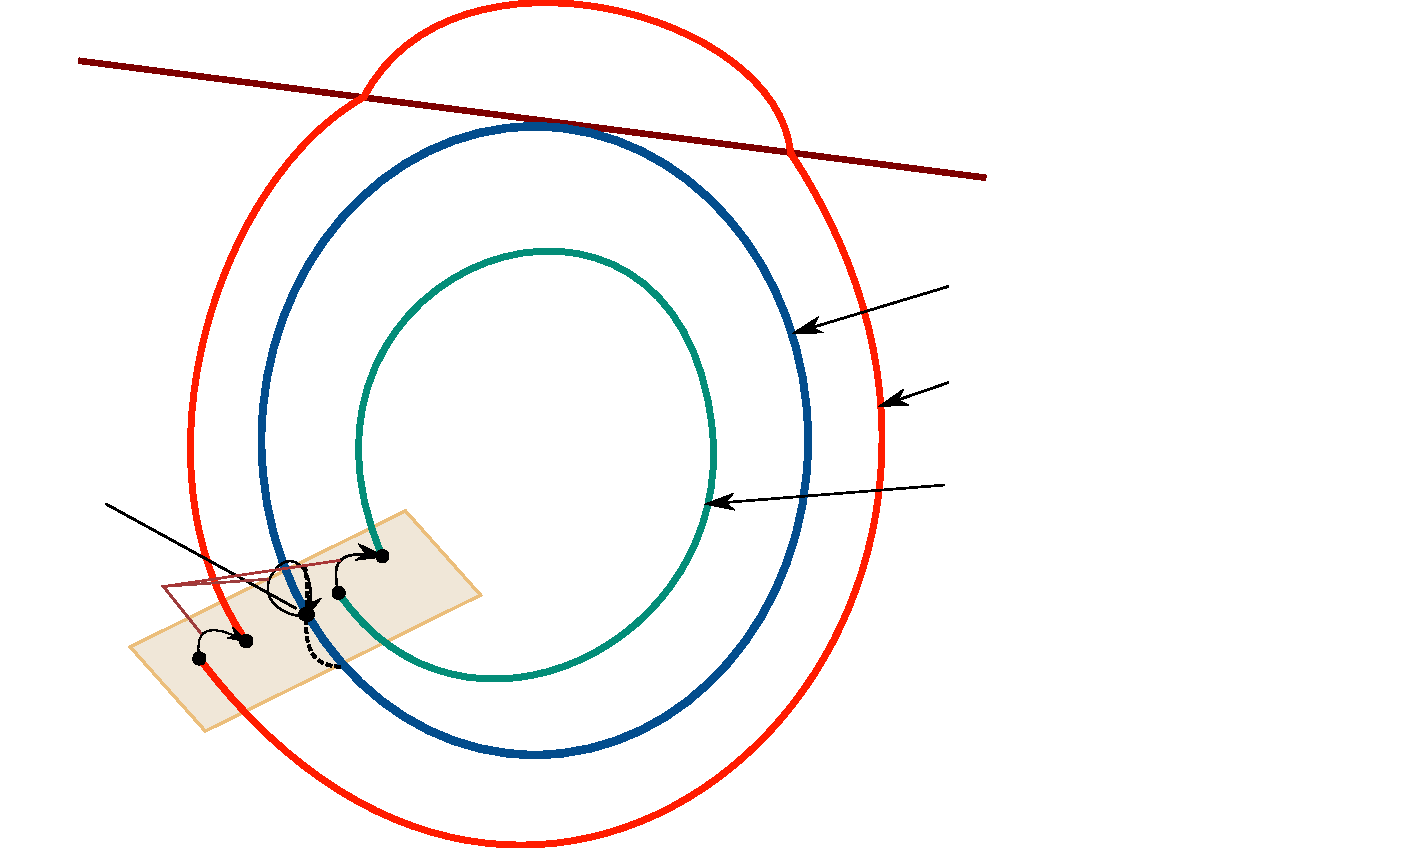
\includegraphics[height=0.45\textheight]{graz}
\end{center}
\end{figure}
\end{frame}

\section{ZDM-existence}
\begin{frame}{Does the ZDM exist?}
\begin{columns}[c]
\column{0.7\textwidth}
\hlb{ Calculate $t_1$:}
Let $T_1(x)$ be the function solving:
\begin{align*}
E_1(x,T_1)&=0\\
\left.  \frac{\partial H(\varphi_1(x,t))}{\partial t}\right|_{T_1(x)}&=0\\
\frac{dH}{dx}(\varphi_1(x,t))\frac{\partial\varphi_1(x,t)}{\partial t}\left.  \right|_{T_1(x)}&=0\\
\frac{dH}{dx}(\varphi_1(x,t))F_1(x,T_1(x))&=0\\
\end{align*}
and 
\begin{equation}
\label{impl1}
T_1(0)=0
\end{equation}

\hlb{ Question: Can such a function ever be found?}



\column{0.3\textwidth}
\begin{center}
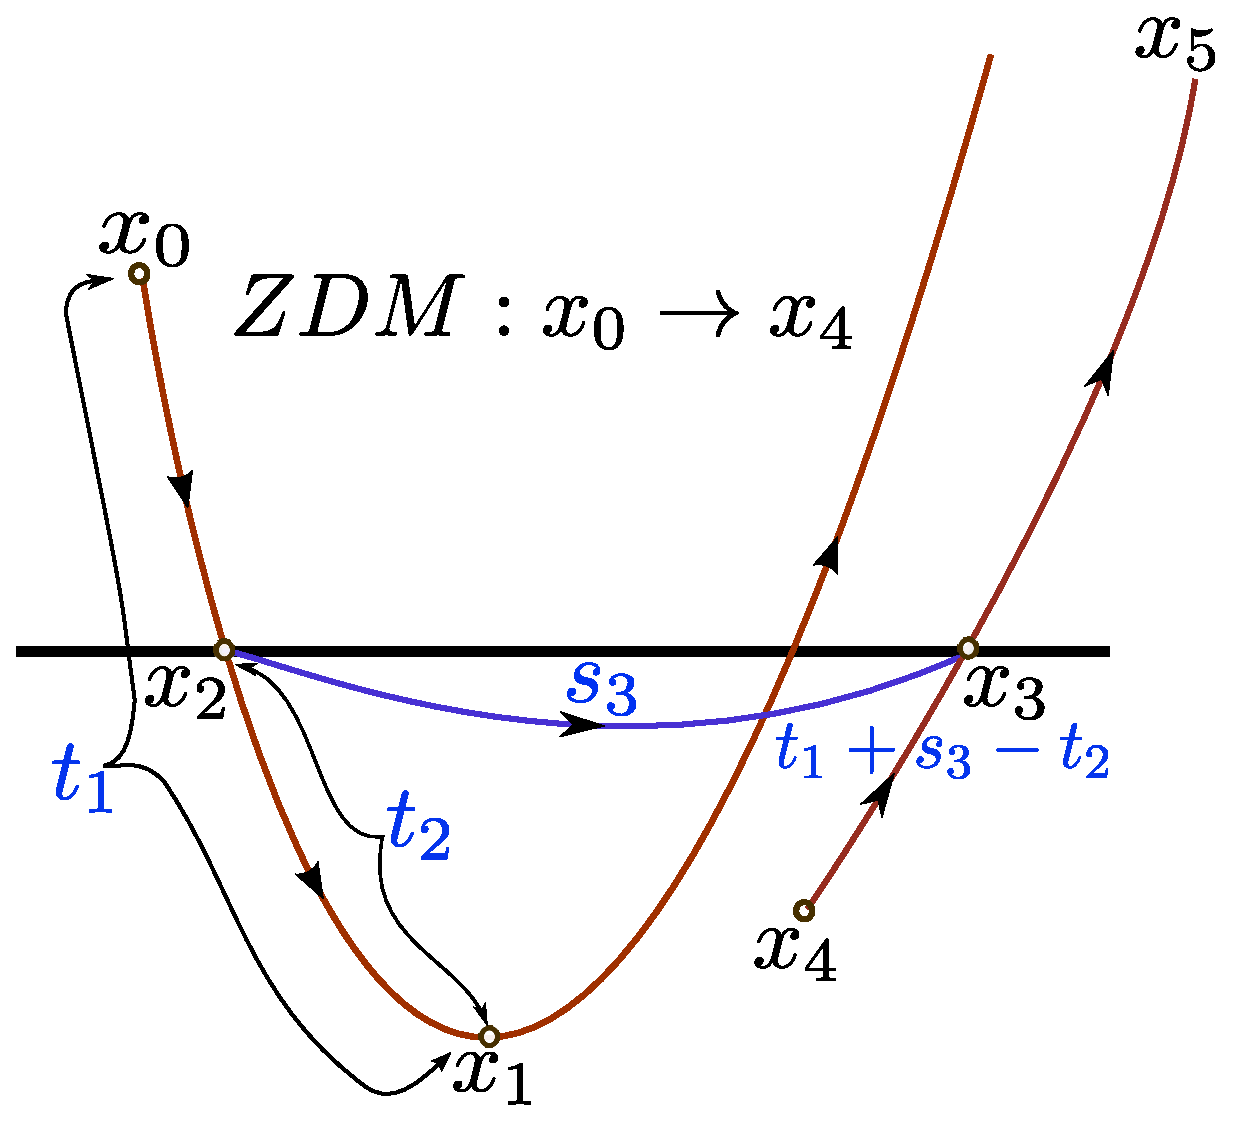
\includegraphics[width=\textwidth]{ZDM}
\end{center}
\end{columns}
\end{frame}


\begin{frame}
\begin{columns}[c]
\column{0.7\textwidth}
\hlb{ Answer: Implicit function theorem}\\


Given any equation $f(x,y)=0$, an explicit function $y=y(x)$ can always be 
found \hl{ in the neighbourhood} of a point $(x_0,y_0)$ satisfying $f(x_0,y_0)=0$
if:
\[
\left.  \frac{\partial f}{\partial y}\right|_{(x_0,y_0)}\neq 0
\]

\pause{}
In other words, $y=y(x)$ can always be found if $y=y(x)$ exists!

\column{0.3\textwidth}
\begin{center}
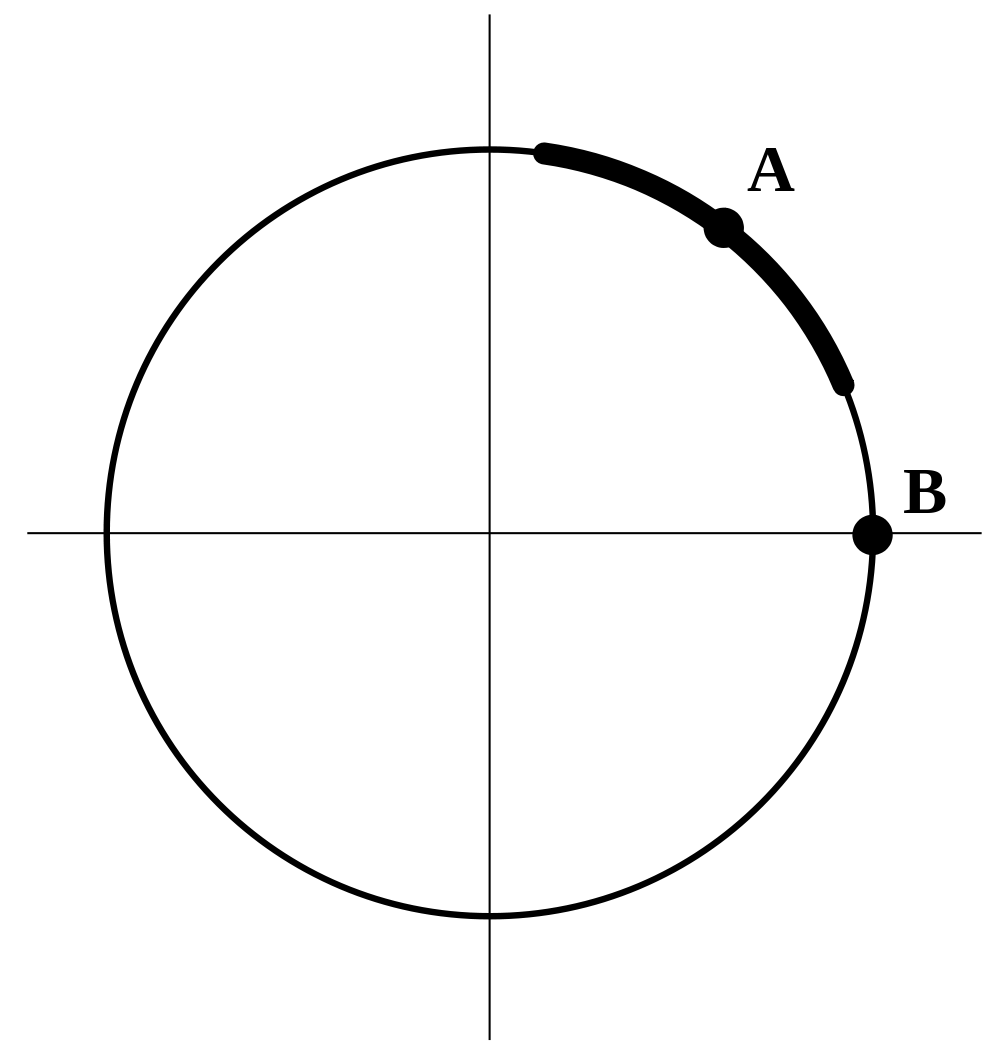
\includegraphics[width=\textwidth]{implicit_circle}
\end{center}
\begin{align*}
f(x,y)&=x^2+y^2-1\\
\left.  \frac{\partial f}{\partial y}\right|_{(x_0,y_0)}&=2y_0
\end{align*}
\end{columns}
\end{frame}


\begin{frame}
\begin{columns}[c]
\column{0.7\textwidth}
Now, in case of \eqref{impl1}, $T_1(x)$ will be found if:
\[
\frac{\partial E_1}{\partial t}(0,0)=\frac{\partial^2}{\partial t^2}\left.  
H(\varphi_i(x,t))\right|_{0,0}=a_i\neq 0
\]
\\

But that was the last criterion of our grazing orbit!\\
\vspace{1em}

So, $T_1(x)$ can be found and $H_{min}(x)=H(\varphi_1(x_0,T_1(x_0)))=H(x_1)$ 
is the minimum value of $H$ that can possibly be found in a travectory 
starting with $x_0$ (Completely disregarding the boundary.  )\\

\column{0.3\textwidth}
\begin{center}
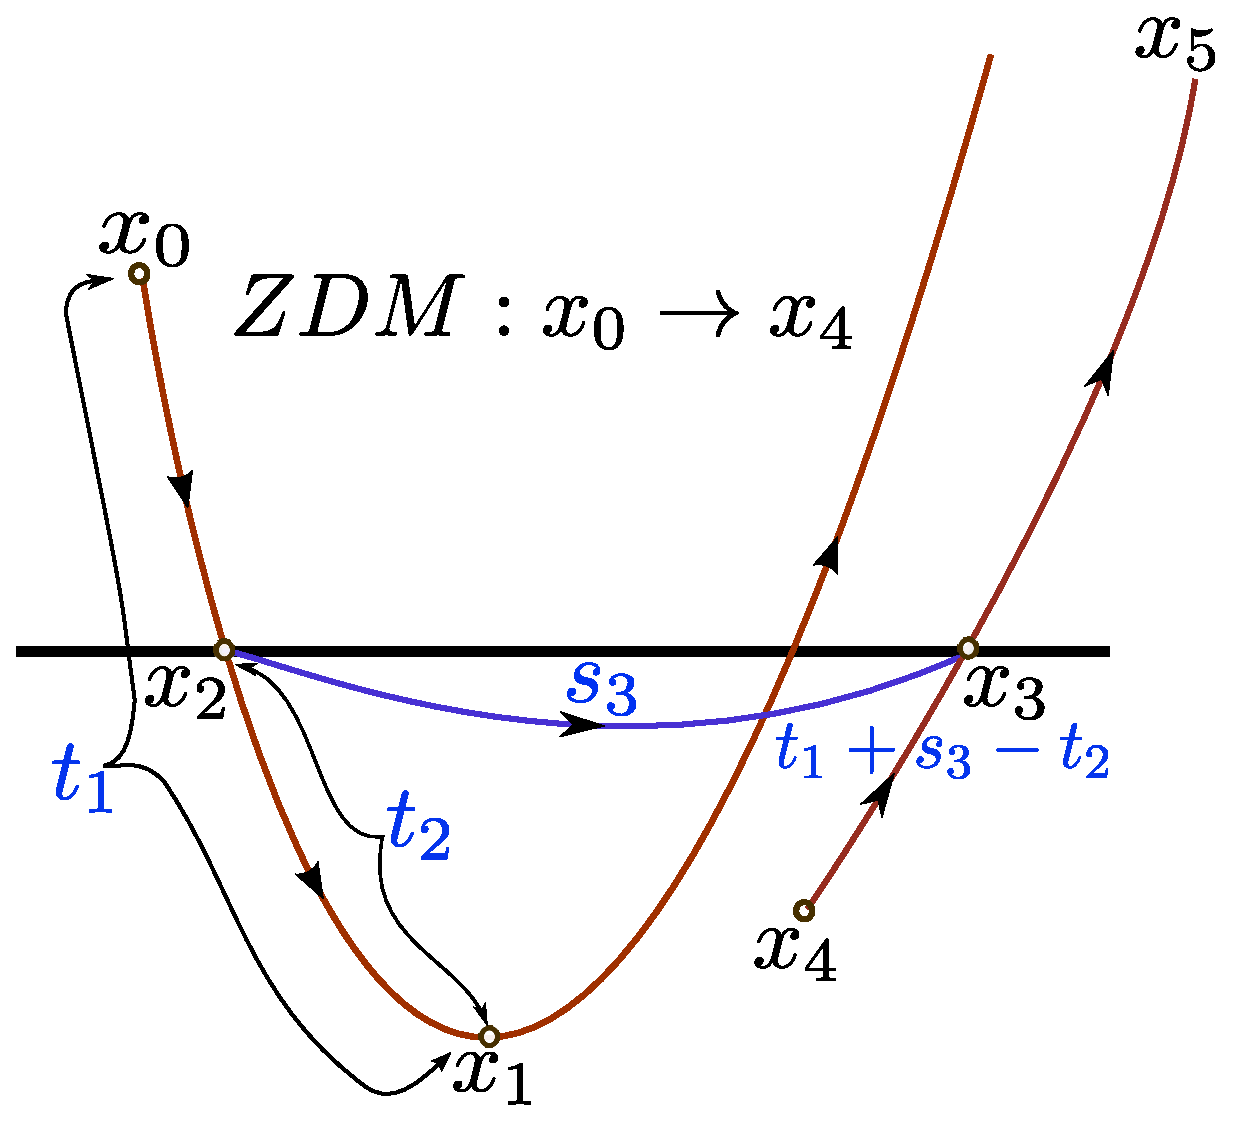
\includegraphics[width=\textwidth]{ZDM}
\end{center}

\end{columns}
\end{frame}


\begin{frame}
\begin{columns}[c]
\column{0.7\textwidth}
\hlb{ Calculate $t_2$:}
Can we do the same trick and extract $t_2$?.\\
\vspace{1em}
\hlb{ Attempt 1: }$H(\varphi_1(x_1,-T_2(x_1)))=0$ close to $T_2(0)=0$.  \\

\vspace{1em}

\hlb{ IFT not applicable} because there are multiple values of $T_2$.  

\vspace{1em}
\hlb{ Attempt 2: } Solve for $E_2(x,y,T_2)$ given by:
\[
T_2\sqrt{\frac{H(\varphi_1(x,T_1(x)-T_2))-H(\varphi_1(x,T_1(x)))}{T_2^2}}-y=0
\]

Around $(0,0,0)$.  \\
$t_2=T_2(x_0,\sqrt(-H_{min}(x_0)))$
\\


\column{0.3\textwidth}
\begin{center}
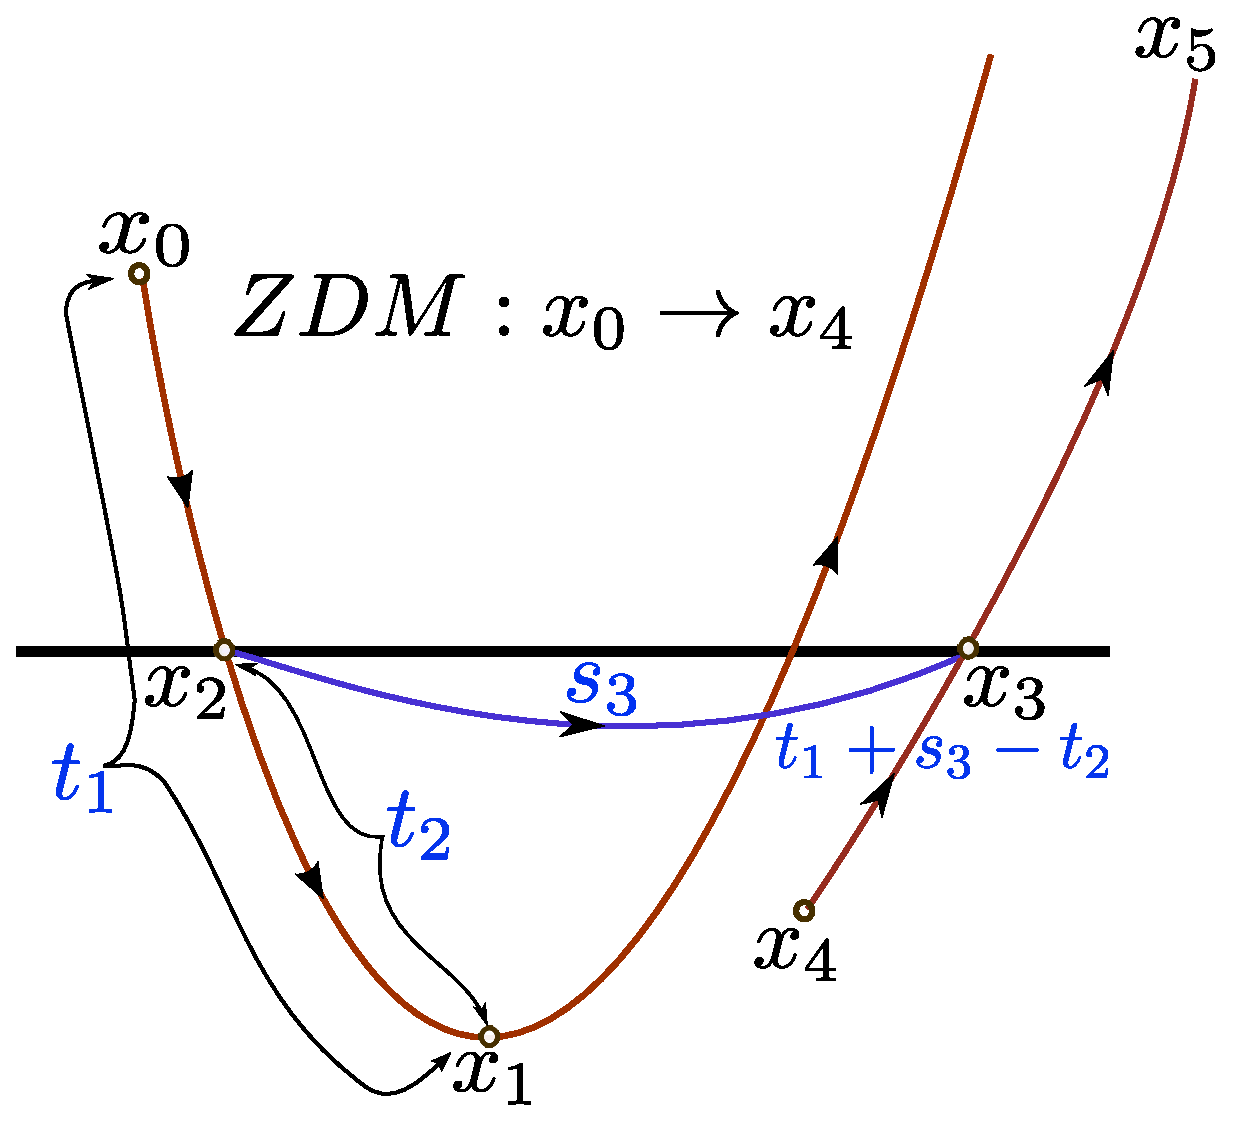
\includegraphics[width=\textwidth]{ZDM}
\end{center}

\end{columns}
\end{frame}

\begin{frame}
\begin{columns}[c]
\column{0.7\textwidth}
\hlb{ Calculate $s_3$:}\\
\[
E_3(x,S_3)=\frac{H(\varphi_2(x,s_3))-H(x)}{s_3}=0
\]
Near $(0,0)$.  \\

$s_3=S_3(x_2)$


\vspace{1em}
(Again manipulated to remove one root)\\

\vspace{1em}
This proves that ZDM exists.  
\column{0.3\textwidth}
\begin{center}
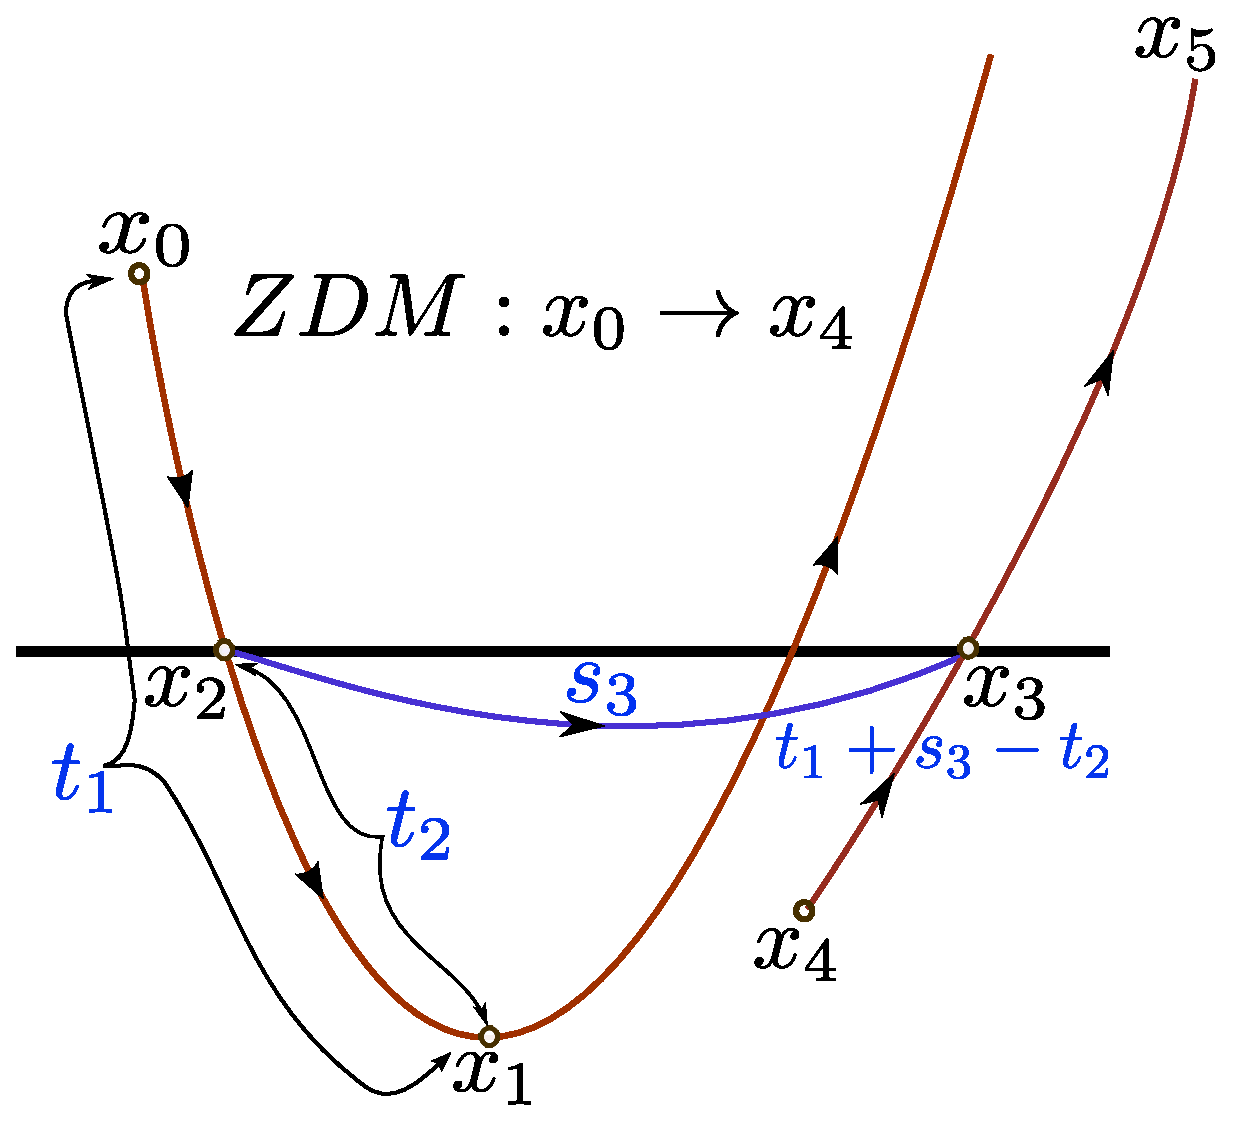
\includegraphics[width=\textwidth]{ZDM}
\end{center}

\end{columns}
\end{frame}

\section{ZDM-calculation}
\begin{frame}{Actually calculating it}
\begin{columns}[c]
\column{0.7\textwidth}
\hl{First intersection:}
\begin{align*}
x_1&\approx x_i+\frac{\partial \varphi_1(x,t)}{\partial t}\left.  \right|_{(x_i,0)}\delta_0\\
&= x_i+F_1(x_i)\delta_0
\end{align*}

Upto 1st order:
\begin{equation}
\label{eq-d0}
x_1=x_i+F_1^*\delta_0
\end{equation}

$F^*:=F(x)|_{x^*}$\\

\column{0.3\textwidth}
\begin{center}
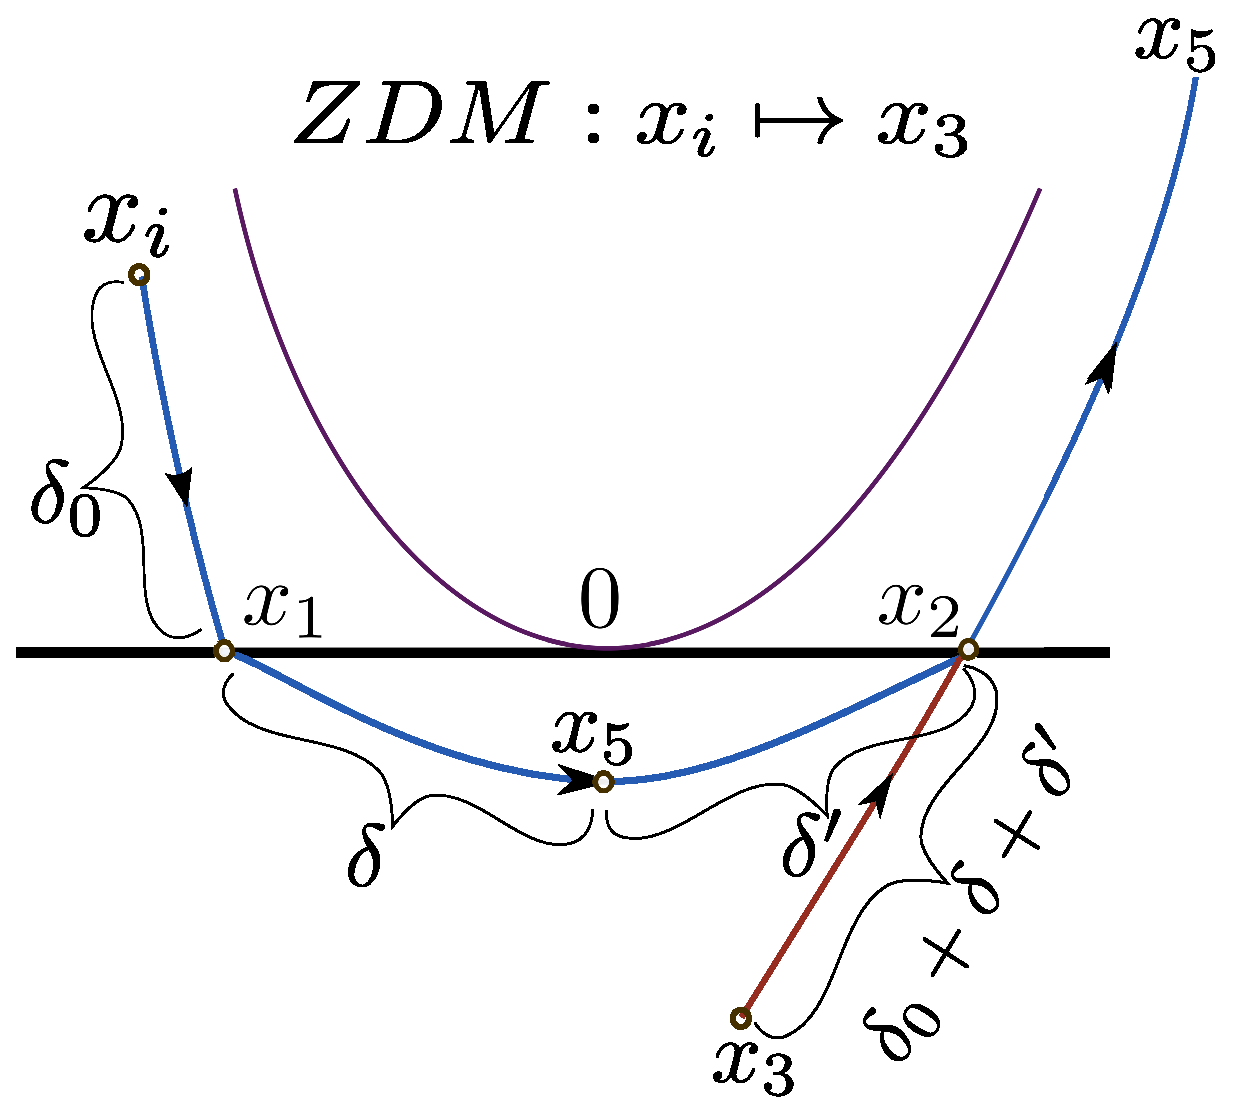
\includegraphics[width=\textwidth]{ZDM_eval}
\end{center}

\end{columns}
\end{frame}

\begin{frame}
\begin{columns}[c]
\column{0.7\textwidth}
\hlb{Calculate $\delta$:}
\begin{align*}
H(x_1)&=H(\varphi(x_5,-\delta))\\
&\approx H(\varphi_2(x_5,0))+\frac{\partial}{\partial t}H(\varphi_2(t,x_5))\left.  
\right|_{t=0}(-\delta)\\
&+\frac{\partial^2}{\partial t^2}H(\varphi_2(t,x_5))\left.\right|_{t\approx0}\frac{\delta^2}{2}\\
&\approx H(x_5)+\frac{\partial^2}{\partial t^2}H(\varphi_2(t,0))\left.\right|_{t\approx0}\frac{\delta^2}{2}\\
&\approx H(x_5)+a_2^*\frac{\delta^2}{2}
\end{align*}

Let $H(x_5)=H_{min}(x_i)=-y^2:$ 
\begin{equation}
\label{eq-d}
\delta=y\sqrt{\frac{2}{a_2^*}}
\end{equation}

\column{0.3\textwidth}
\begin{center}
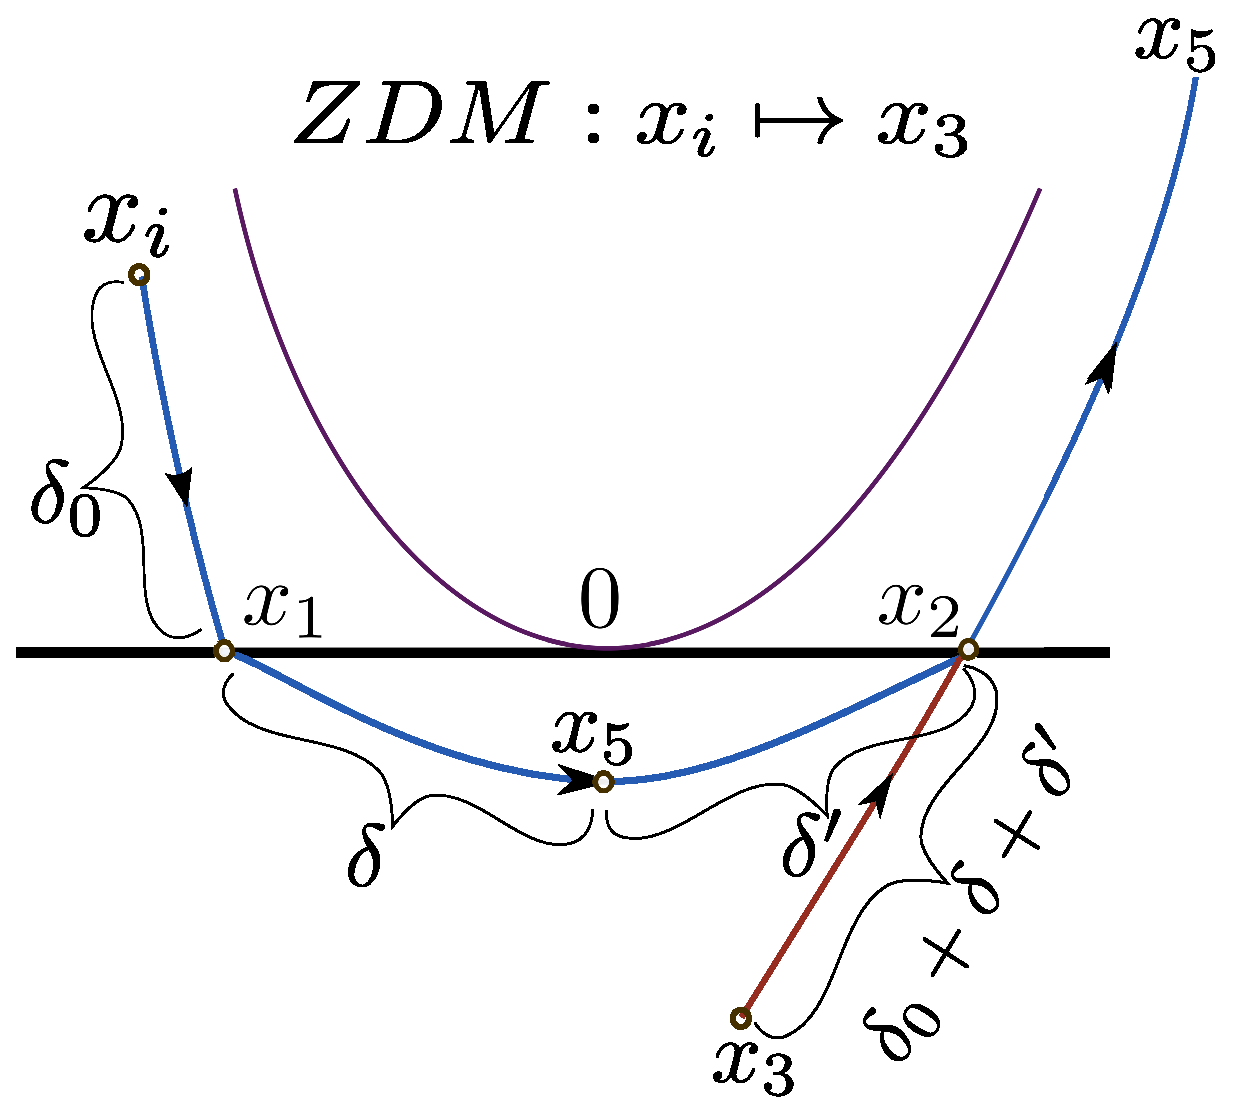
\includegraphics[width=\textwidth]{ZDM_eval}
\end{center}

\end{columns}
\end{frame}


\begin{frame}
\begin{columns}[c]
\column{0.7\textwidth}
\hlb{Calculate ZDM:}
Using identical arguments, $\delta^{\prime}=y\sqrt{\frac{2}{a_2^*}}$ \\
Let $\delta+\delta^{\prime}=\delta_1$

Then:
\begin{align}
\label{final}
x3&\approx x_2-F_1(x_2)\delta_1+\dot{F_1}(x_2)\frac{\delta_1^2}{2}-\ddot{F_1}(x_2)\frac{\delta_1^3}{6}\\
x1&\approx x_2-F_2(x_2)\delta_1+\dot{F_2}(x_2)\frac{\delta_1^2}{2}-\ddot{F_2}(x_2)\frac{\delta_1^3}{6}
\end{align}

\begin{equation}
\label{zdm-final}
x_3=x_1-(F_1-F_2)(x_2)\delta_1+(\dot{F_1}-\dot{F_2})(x_2)\frac{\delta_1^2}{2}-(\ddot{F_1}-\ddot{F_2})(x_2)\frac{\delta_1^3}{6}
\end{equation}
\column{0.3\textwidth}
\begin{center}
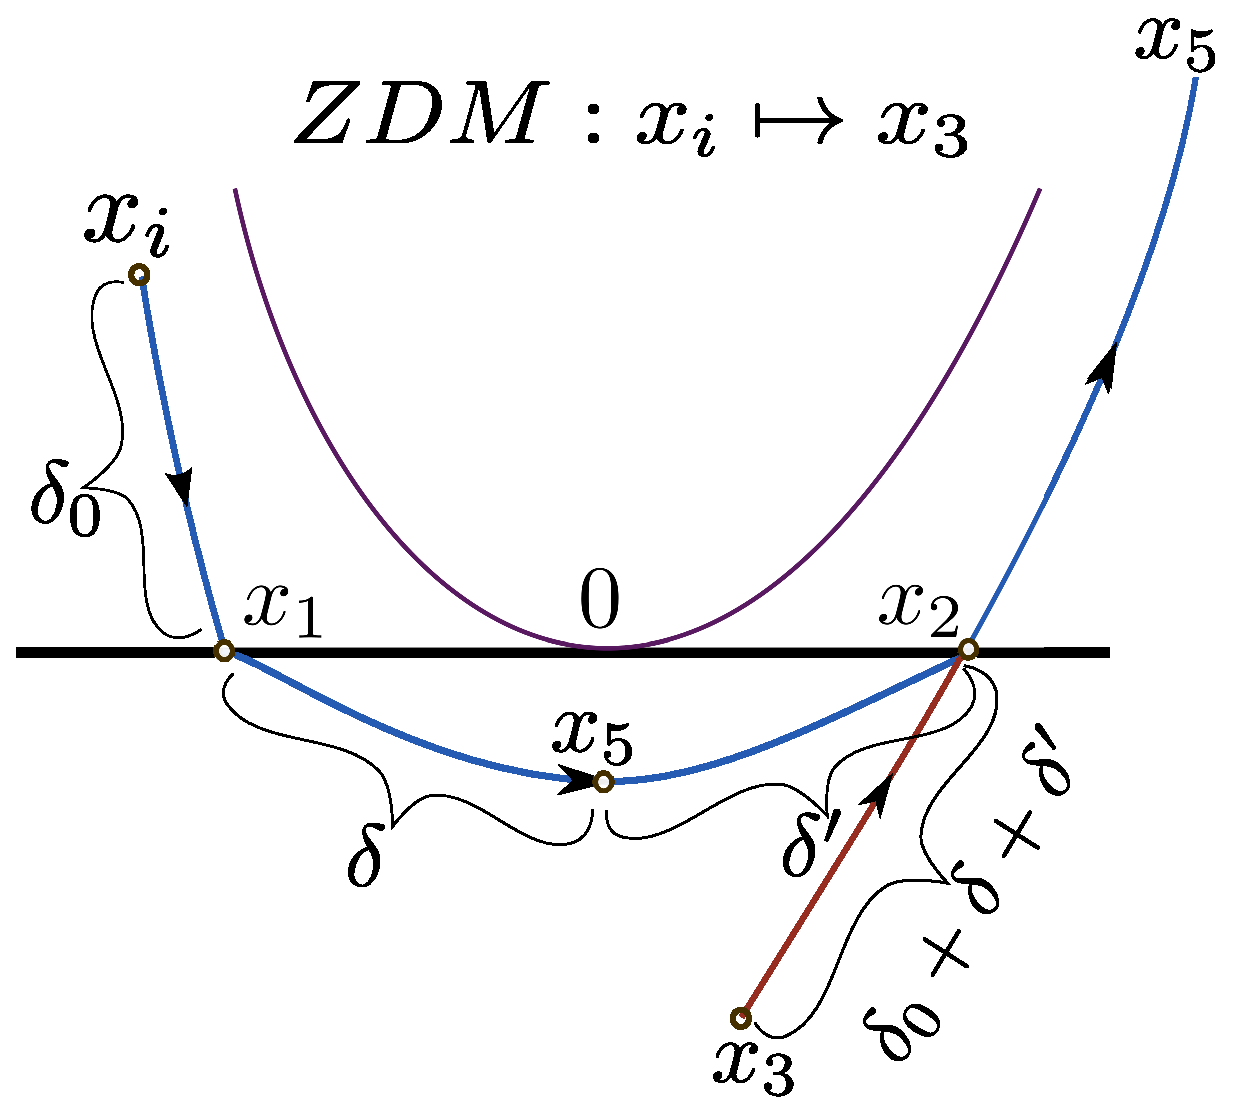
\includegraphics[width=\textwidth]{ZDM_eval}
\end{center}
\end{columns}
\end{frame}

\begin{frame}
\hlb{A system with discontinuous first derivative:}
\begin{columns}[c]
\column{0.7\textwidth}
\begin{align}
\label{}
F_1(x)&=F(x)\\
F_2(x)&=F(x)+GH(x)
\end{align}

Then, ignoring the spatial derivatives of $H(x)$:
\begin{align*}
(F_1-F_2)(x_2)&\approx (F_1-F_2)(x^*)\\
&=GH(0)\\
&=0\\
(\dot{F_1}-\dot{F_2})(x_2)&=G\dot{H}(0)\\
&=0\\
(\ddot{F_1}-\ddot{F_2})(x_2)&=G\ddot{H}(0)\\
&=Ga^*
\end{align*}
\column{0.3\textwidth}
\begin{center}
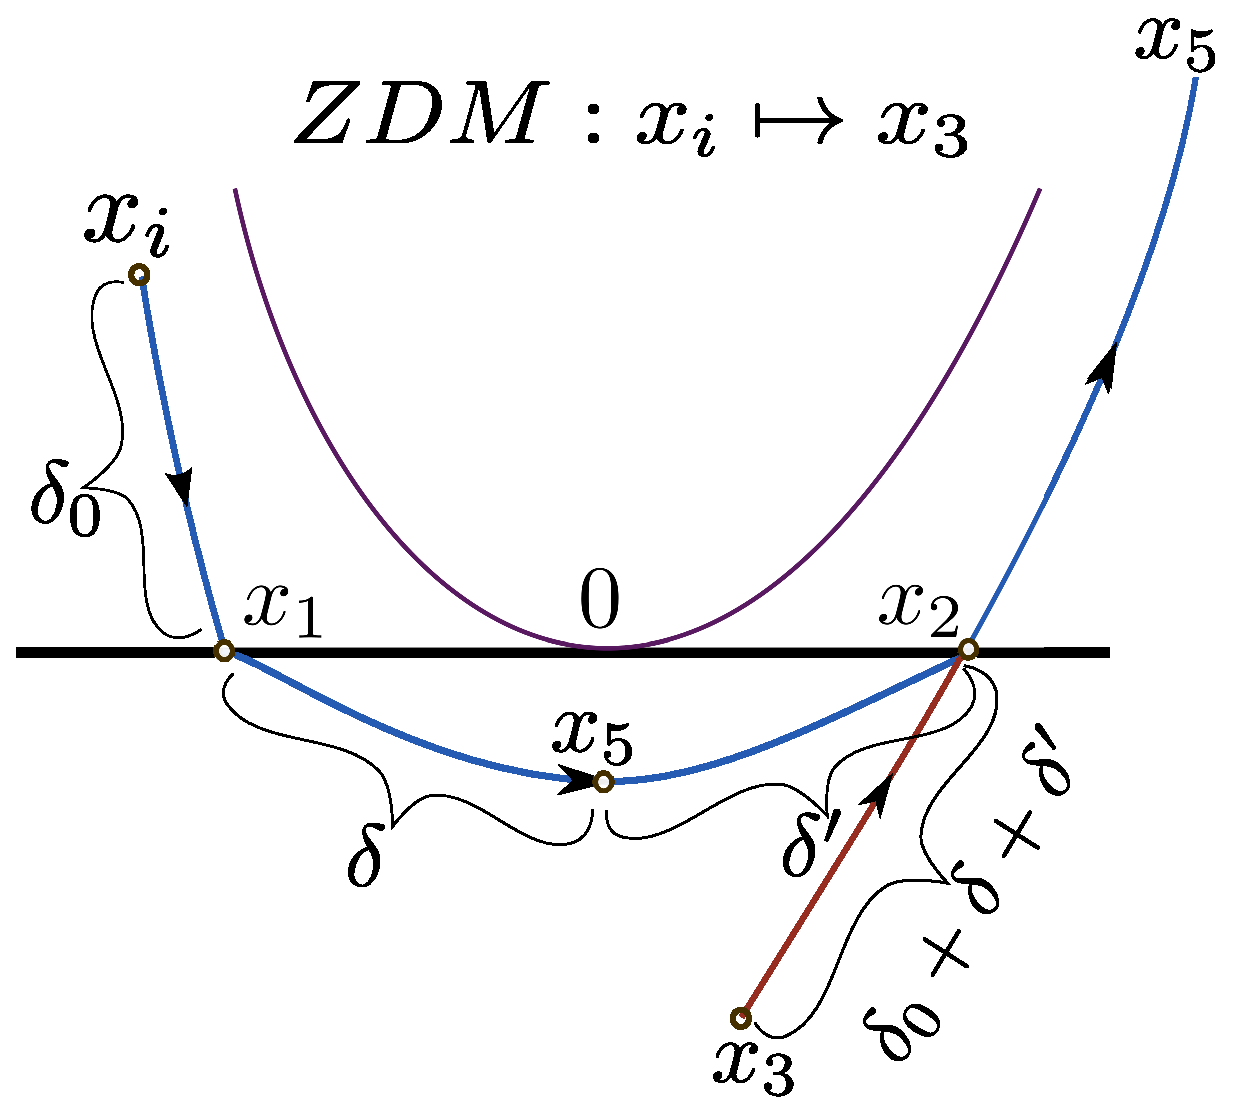
\includegraphics[width=\textwidth]{ZDM_eval}
\end{center}

\[
x_3=x_i+\frac{8}{3}G\sqrt{\frac{2}{a^*}}y(x_i)^3
\]


\end{columns}
\end{frame}

\begin{frame}{General form of ZDM}
\begin{columns}[c]
\column{0.7\textwidth}
\hlb{Evaluating $t_2$}
\begin{align*}
0=&H(\varphi_1(x_1,t_2))\\
0=&H(\varphi_1(x_1,t_2))-(y^2+H(x_1))-\lie{F_1}H(x_1)t_2&\\
0\approx&H(x_1)+\lie{F_1}H(x_1)t_2+\lien{F_1}{2}H(x_1)\frac{t_2^2}{2}+\\&\lien{F_1}{3}H(x_1)\frac{t_2^3}{6}-y^2-H(x_1)-\lie{F_1}H(x_1)t_2\\
0\approx&\lien{F_1}{2}H(x_1)\frac{t_2^2}{2}+\lien{F_1}{3}H(x_1)\frac{t_2^3}{6}-y^2
\end{align*}

It can be argued from IFT that $t_2(x_1,y)$ can be expressed as apower series:
\[
t_2=A(x_1)y+B(x_1)y^2+O(y^3)
\]
\column{0.3\textwidth}
\begin{center}
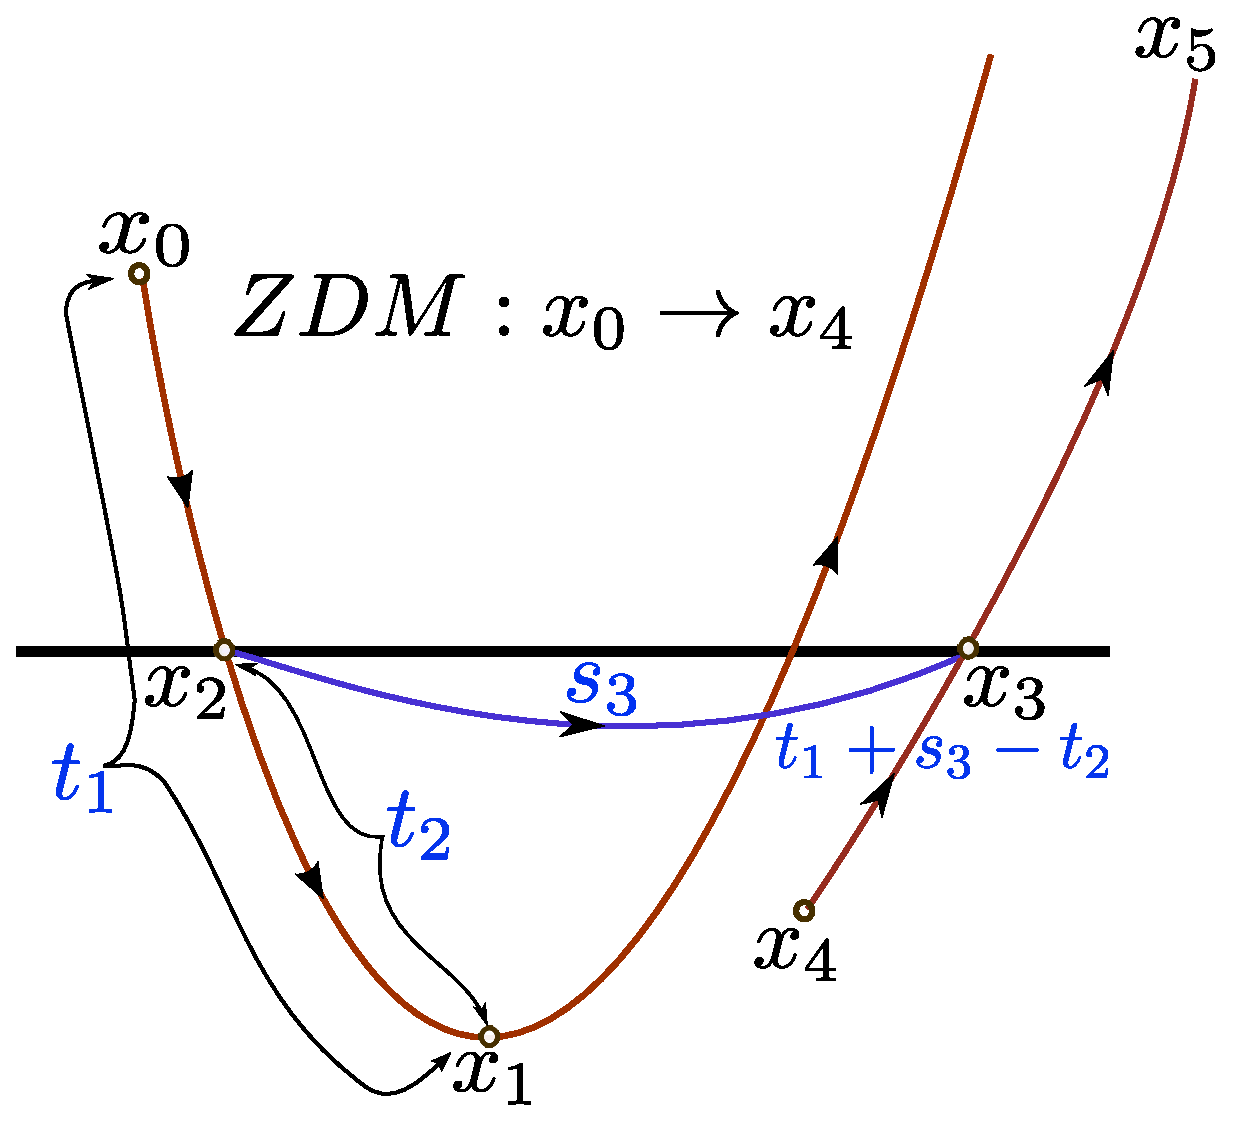
\includegraphics[width=\textwidth]{ZDM}
\end{center}
\end{columns}
\end{frame}


\begin{frame}{General form of ZDM}
\begin{columns}[c]
\column{0.7\textwidth}
The coefficients $A,B$ are easily computed:
\begin{equation}
\label{eq-t2}
t_2(x_1,y)=-\sqrt{\frac{2}{\lien{F_1}{2}H(x_1)}}y-\frac{1}{3}\frac{\lien{F_1}{3}H(x_1)}{(\lien{F_1}{2}H(x))^2}y^2+O(y^3)
\end{equation}
There are multiple 
solutions, use the constraint $t_2<0$ to eliminate spurious ones

\hlb{Evaluating $s_3$}\\
\begin{align*}
H(\varphi_2(x_2,s_3))=&0\\
\lie{F_2}H(x_2)s_3+\lien{F_2}{2}\frac{s_3^2}{2}\approx&0
\end{align*}

Now put $x_2=\varphi_1(x_1,t_2)$ and Taylor expand:

\column{0.3\textwidth}
\begin{center}
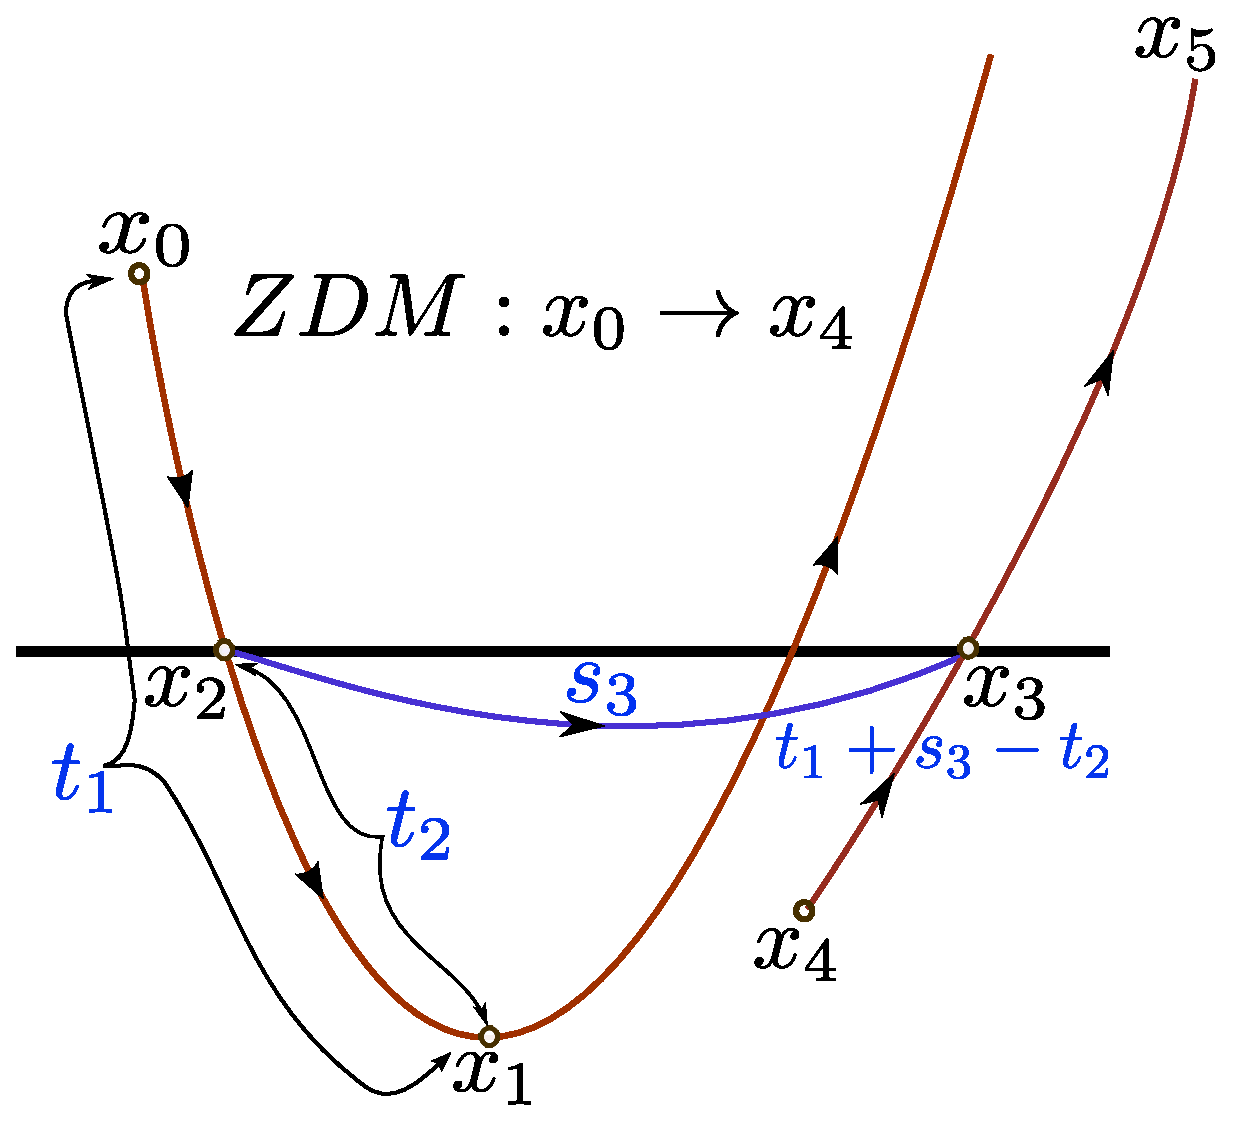
\includegraphics[width=\textwidth]{ZDM}
\end{center}
\end{columns}
\end{frame}

\begin{frame}{General form of ZDM}
\begin{columns}[c]
\column{0.7\textwidth}
\[
\lie{F_2}H(x_1)s_3-C(x_1)\lie{F_1}\lie{F_2}H(x_1)ys_3+\frac{1}{2}\lien{F_1}{2}H(x_1)s_3^2+O(s_3^3)=0
\]

Where $C(x)=\sqrt{\frac{2}{\lien{F_1}{2}H(x)}}$.  \\
\pause{}
Note that $\lie{F_2}H(x_1)$ should be zero because $\lie{F_1}H(x_1)=0$  and to 
prevent sliding the lie derivatives of the two flows must have same sign in 
close neighbourhoods of the boundary.  \\
\pause{}
Now the non-zero solution for $t_3$ is easily obtained:
\begin{equation}
\label{eq-s3}
s_3(x_1,y)=2\frac{\lie{F_1}\lie{F_2}H(x_1)}{\lien{F_2}{2}H(x_1)}C(x_1)y+O(y^2)
\end{equation}

\column{0.3\textwidth}
\begin{center}
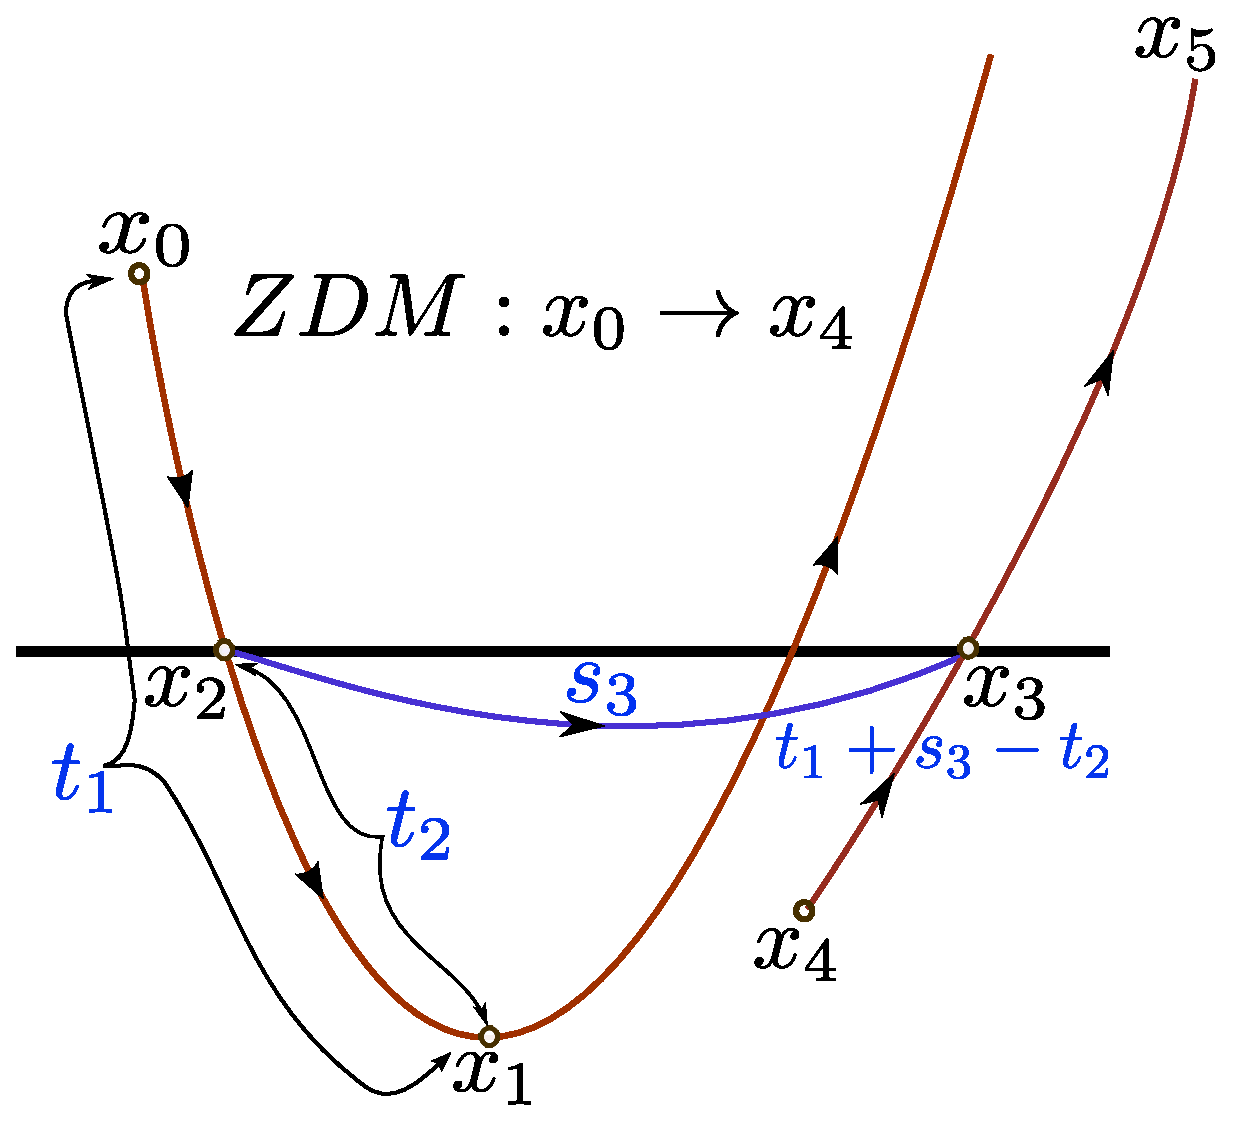
\includegraphics[width=\textwidth]{ZDM}
\end{center}
\end{columns}
\end{frame}

\begin{frame}{General form of ZDM}
\begin{columns}[c]
\column{0.7\textwidth}
\begin{align*}
ZDM(x_1)=&\varphi_1(\varphi_2(\varphi_1(x_1,t_2),s_3),-t_2-s_3)\\
=&\varphi_1(\varphi_2(x_1+F_1t_2,s_3),-t_2-s_3)+O(s_3^2)\\
=&\varphi_1(x_1+F_1t_2+F_2s_3,-t_2-s_3)+O((s_3,t_2)^2)\\
=&x_1+F_1t_2+F_2s_3-F_1(t_2+s_3)+O((s_3,t_2)^2)\\
=&x_1+s_3(F_2-F_1)(x_1)+O((s_3,t_2)^2)\\
\approx&x_1+2\frac{\lie{F_1}\lie{F_2}H(x_1)}{\lien{F_2}{2}H(x_1)}y\sqrt{\frac{2}{\lien{F_1}{2}H(x)}}(F_2-F_1)(x_1)
\end{align*}

Where $y=\sqrt{-H(x_1)}$.  
But in general, we need $ZDM(x_0)$.  
\column{0.3\textwidth}
\begin{center}
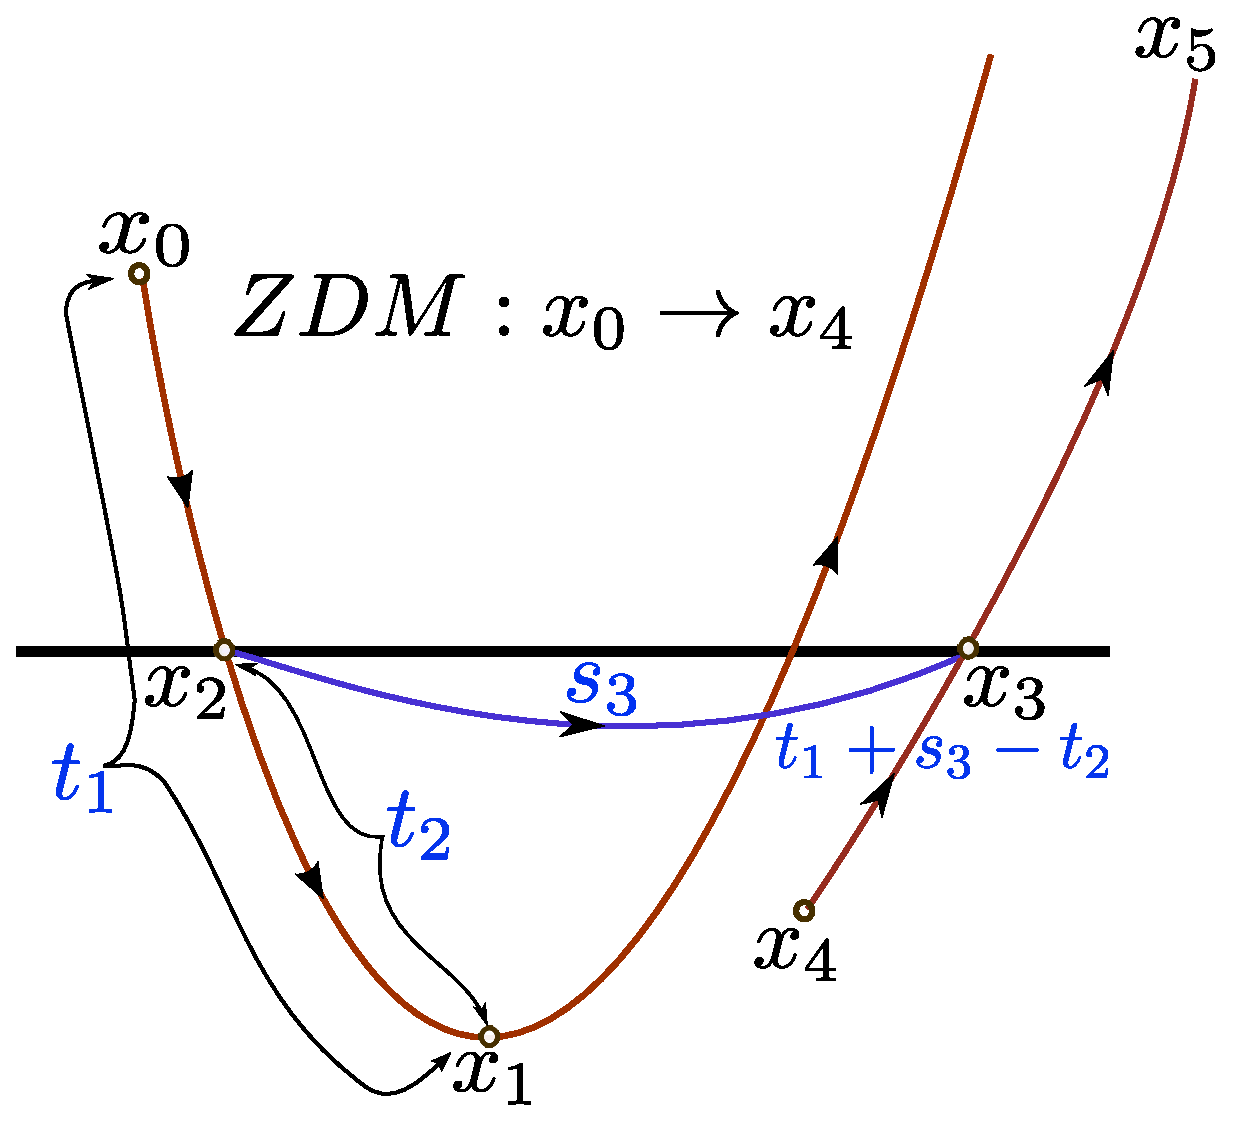
\includegraphics[width=\textwidth]{ZDM}
\end{center}
\end{columns}
\end{frame}

\begin{frame}{General form of ZDM}
\begin{columns}[c]
\column{0.7\textwidth}
Have to solve for $t_1$:\\
\begin{align*}
\lie{F_1}H(\varphi_1(x_0,t_1))=&0\\
\lie{F_1}H(x_0)+\lien{F_1}{2}H(x_0)t_1=&0\\
\rightarrow t_1=&-\frac{\lie{F_1}H(x_0)}{\lien{F_1}{2}H(x_0)}
\end{align*}

\begin{align}
\label{eq-hmin}
H_{min}(x)=&H(\varphi_1(x,t_1(x)))\\
=&H(x)+\lie{F_1}H(x)t_1(x)\\
=&H(x)-\frac{(\lie{F_1}H(x_0))^2}{\lien{F_1}{2}H(x_0)}
\end{align}


\column{0.3\textwidth}
\begin{center}
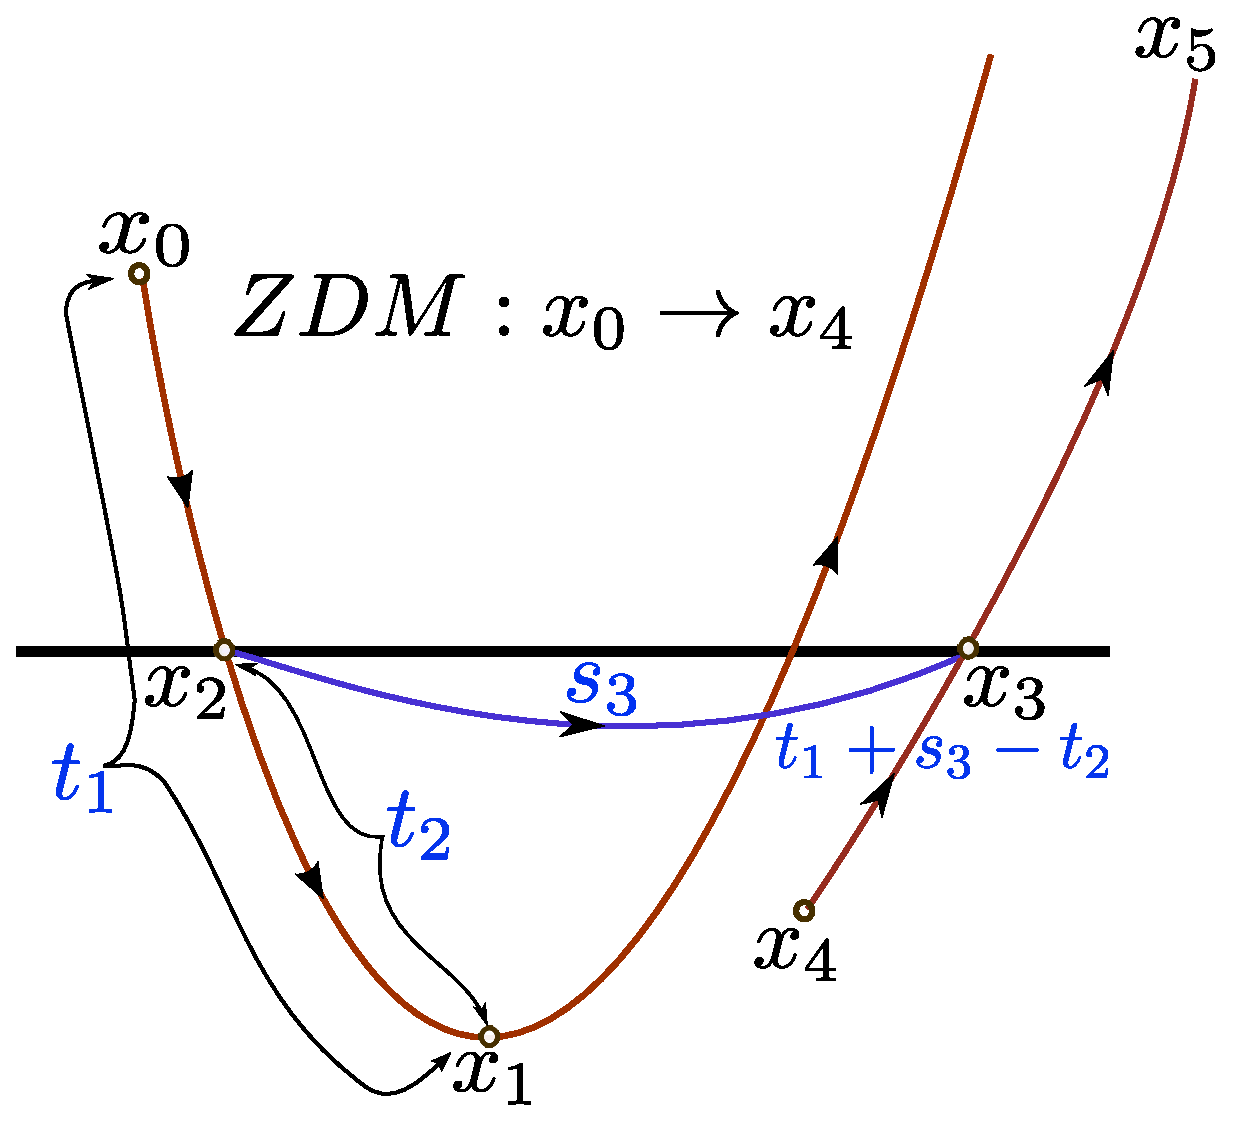
\includegraphics[width=\textwidth]{ZDM}
\end{center}
\end{columns}
\end{frame}


\begin{frame}{General form of ZDM}
\begin{columns}[c]
\column{0.7\textwidth}
\begin{align*}
ZDM(x_0)=&\varphi_1(\varphi_2(\varphi_1(x_0,t_1+t_2),s_3),-t_1-t_2-s_3)\\
\approx&x_0+2\frac{\lie{F_1}\lie{F_2}H(x_1)}{\lien{F_2}{2}H(x_1)}y\sqrt{\frac{2}{\lien{F_1}{2}H(x)}}(F_2-F_1)(x_1)
\end{align*}

Where $y=\sqrt{-H(x)+\frac{(\lie{F_1}H(x_0))^2}{\lien{F_1}{2}H(x_0)}}$.  

Since we are keeping terms only upto the $1$st order of the small parameter(
$s_3$), we can evaluate all functions at the grazing point $x^*$ instead of 
$x_1$, provided $|x^*-x_1|\approx0$ 

\column{0.3\textwidth}
\begin{center}
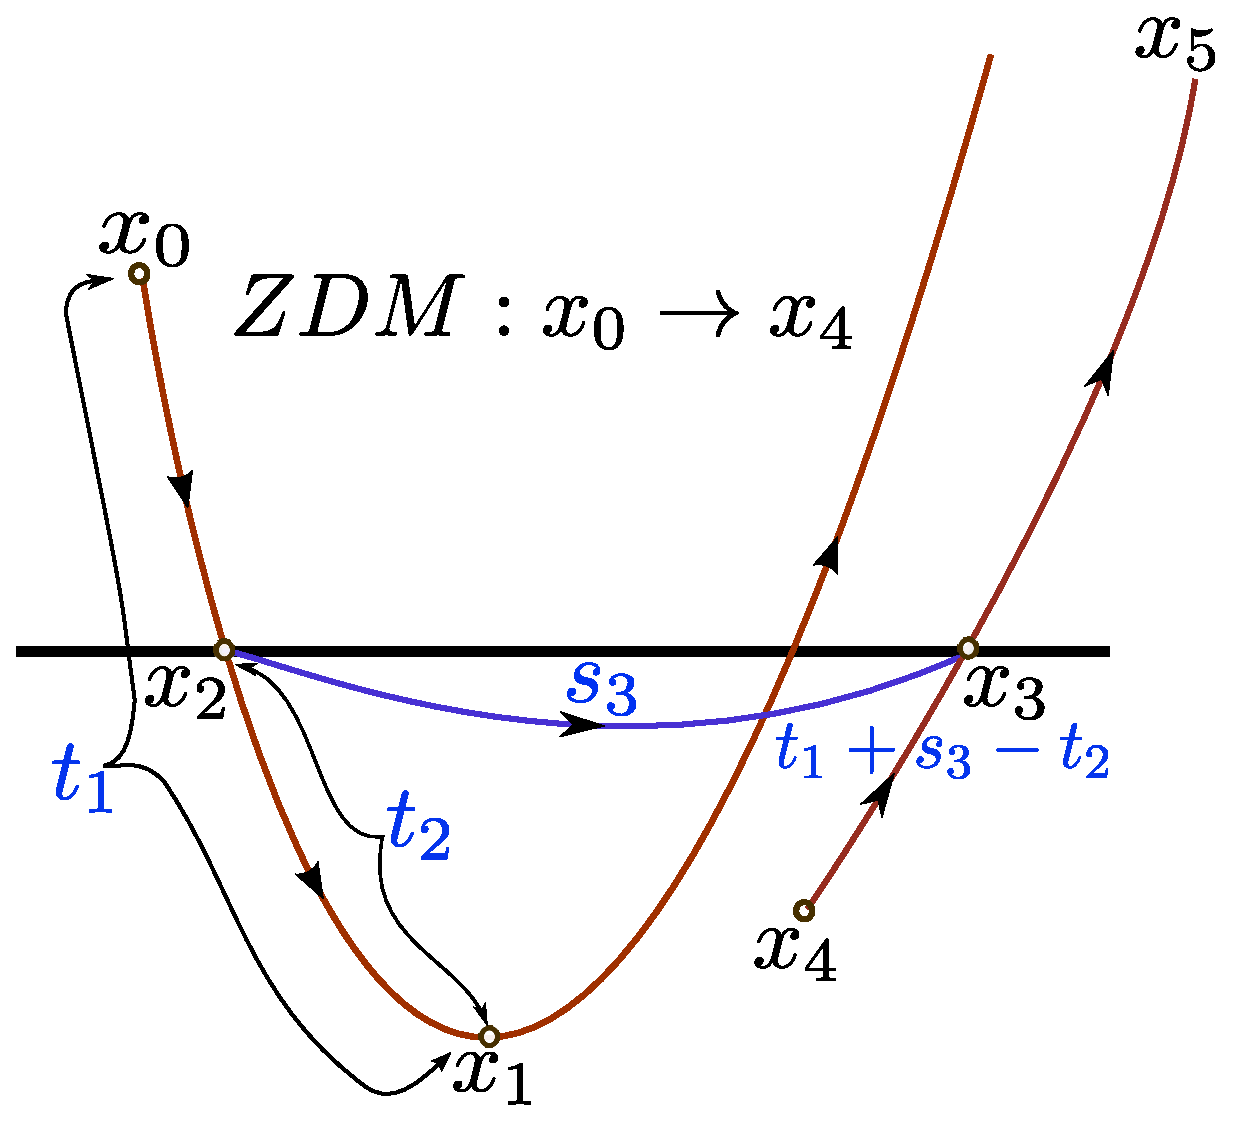
\includegraphics[width=\textwidth]{ZDM}
\end{center}
\end{columns}
\end{frame}

\begin{frame}{The case of discontinuous first derivative}
\hlb{What if $(F_2-F_1)x^*=0$?}
Then of course, the leading order term in the discontinuity map will be 
\emph{2nd order} in the small parameters $t_1,t_2, s_3$. Consequentially, we 
must evaluate those parameters upto $2nd$ order themselves.  

\end{frame}


\begin{frame}{The case of discontinuous first derivative}

We will see that it will involve leading order discontinuity term of order 
$O(y^3)=O(|x|^3/2)$.  

The procedure is identical, only upto higher 
order:

\begin{align*}
ZDM(x_0)=&\varphi_1(\varphi_2(\varphi_1(x_0,t_1+t_2),s_3),-t_1-t_2-s_3)\\
\end{align*}

\begin{align*}
\varphi_1(x_0,t_1+t_2)&\approx x_0+F_1(x_0)(t_1+t_2)+\frac{dF_1(x_0)}{dt}(t_1+t_2)\\&+\frac{d^2F_1(x_0)}{dt^2}(t_1+t_2)^2/2+\frac{d^3F_1(x_0)}{dt^3}(t_1+t_2)^3/6
\end{align*}

Ultimately we get: $ZDM(x_0)=P(x_0,t_1,t_2,s_3)+O(t_1^4,t_2^4,s_3^4)$.  

Next, we need to re-evaluate  $t_1,t_2$ upto order $y^3$ and replace in the 
formula for $ZDM$. That completes the job.   
\end{frame}

\begin{frame}{Poincare map}
\[
X_{n+1}}=  (N_2 \cdot ZDM \cdot N_1) X_n = P(X_n)
\]

The trace and/or determinant of $P$ will show the discontinuity of ZDM.  The 
determinants will determine the stability of orbits.  

\end{frame}


\end{document}
